\documentclass[14pt,a4]{article}

\usepackage{amsmath}
\usepackage{enumitem}
\usepackage{graphicx}
\usepackage{xcolor}
\usepackage{subcaption}
\usepackage{xepersian}

\settextfont{XB Kayhan}
\setlatinsansfont{Times Newer Roman}

\title{\vspace{-4cm} \textbf{پاسخ تمرینات سری اول درس یادگیری ماشین}}
\author{محمدرضا غفرانی  ۴۰۰۱۳۱۰۷۶}
\date{\today}

\begin{document}

\maketitle

\section*{پرسش‌های تشریحی}

\subsection*{سوال یک}

\begin{enumerate}[label=\alph* )]
    \item نادرست. از آن جا که معمولا کاهش بیش از حد خطا در داده‌های آموزشی منجر به بیش‌برازش می‌شود، در نتیجه
    دانش کسب شده توسط مدل قابل تعمیم به داده‌های ارزیابی نیست و در نتیجه خطای مدل در داده‌های ارزیابی بیشتر می‌شود.
    \item درست. در هنگام یادگیری مدل تلاش می‌کند خطای خود را بر روی داده‌های موجود برای آموزش کم کند. اگر در این
    مرحله تعداد داده‌ی آموزشی کمی در دسترس مدل  باشد مدل به راحتی الگوی موجود بین داده‌ها را (هر چند اشتباه!)
    متوجه شده و خطای خود را در داده‌های آموزشی به حداقل می‌رساند. این در حالی است که الگوی کشف شده توسط مدل
    لزوما قابل تعمیم به سایر داده‌ها نیست.
    \item نادرست. برای مثال فرض کنید توزیع داده‌ها به شکل زیر باشد. واضح است که در این جا استفاده از چندجمله‌ای درجه‌ی
    دو نسبت به چندجمله‌ای درجه یک، بهتر می‌تواند داده‌های آبی و قرمز را از هم تفکیک کند.

    \begin{figure}[h]
        \centering
        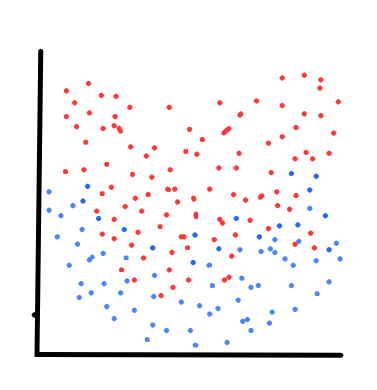
\includegraphics[scale=0.4]{images/q1p3.png}
    \end{figure}
    \item درست. تابع مربوط به هر یک از معیار‌های \lr{MSE}، \lr{RMSE} و \lr{MAE}
    در ادامه آورده شده است. دو معیار \lr{RMSE} و \lr{MSE}
    برای از بین‌بردن مقادیر منفی، همه‌ی مقادیر را به توان دو می‌رسانند.
    در نتیجه اگر داده‌ی پرتی در مجموعه دادگان وجود داشته باشد، این داده در تابع‌های هزینه
    \lr{RMSE} و \lr{MSE} بیش از پیش اثر می‌گذارد. این حرف در رابطه با تابع \lr{MSE} به وضوح درست است اما
    برای تابع \lr{RMSE} به شرح زیر اثبات می‌شود.

    \begin{eqnarray*}
        \text{MAE} & < & \text{RMSE} \\
        \frac{1}{n} \sum_{i=1}^{n} (Y_i - Y'_i) & < & \sqrt{\frac{1}{n} \sum_{i=1}^{n} (Y_i - Y'_i)^2} \\
        \frac{1}{n} \sum_{i=1}^{n} a_i & < & \sqrt{\frac{1}{n} \sum_{i=1}^{n} a_i^2} \\
        \frac{1}{n^2} (\sum_{i=1}^{n} a_i)^2 & < & \frac{1}{n} \sum_{i=1}^{n} a_i^2 \\
        2a_1a_2 + 2a_1a_2 + ... + 2a_ia_j + ... + 2a_{n-1}a_n & < & (n-1) a_1^2 + (n-1) a_2^2 + ... + (n-1) a_n^2
    \end{eqnarray*}
    رابطه بالا به ازای $n$های بزرگ همواره درست است.
\end{enumerate}


\subsection*{سوال دو}

اتفاق رخ داده بیش‌برازش است. برای جلوگیری از این اتفاق از راه‌حل‌های زیر می‌توان استفاده کرد.

\begin{enumerate}
    \item تعداد داده‌ آموزشی را افزایش دهیم.
    \item استفاده از تکنیک‌هایی نظیر \lr{cross validaion}.
    \item ساده‌کردن مدل با کاهش پارامتر‌هایی که باید بهینه کند.
    \item نظم‌دهی یا \lr{regualarization}. بدین معنی که فرمول محاسبه‌ی خطا را به شکل زیر تغییر داده
    و عبارت قرمز را در محاسبه‌ی خطا دخیل کنیم. در این فرمول منظور از $\theta_j$ ضریب جمله‌ با توان $j$
    در چندجمله‌ای است.
    $$E = \frac{1}{2m} \big[ \sum_{i=1}^{n} (Y_i - \hat{Y}_i)^2 \textcolor{red}{+ \sum_{j=0}^{m} \theta_j^2 } \big]$$
\end{enumerate}

\subsection*{سوال سوم}

\subsubsection*{قسمت الف}

ماتریس $X$ و $W$ را به شکل زیر داریم.

$$X = [x_1^T \hspace{0.2cm} x_2^T \hspace{0.2cm} x_3^T \hspace{0.2cm} ...  \hspace{0.2cm} x_n^T]^T$$
$$W = [w_1^T \hspace{0.2cm} w_2^T \hspace{0.2cm} w_3^T \hspace{0.2cm} ...  \hspace{0.2cm} w_n^T]^T$$

حال تابع هزینه را با استفاده از این فرمول بازنویسی می‌کنیم.

\begin{eqnarray*}
    J(W) & = & (XW - y)^T (XW - y) \\
     & = & ((XW)^T - y^T) (XW - y) \\
     & = & (XW)^T(XW) - (XW)^T y - y^T(XW) + y^Ty \\
     & = & (XW)^T(XW) - 2 (XW)^T y + y^Ty \\
\end{eqnarray*}


حال از تابع $J(W)$ نسبت به $W$ مشتق گرفته و مساوی صفر قرار می‌دهیم.

\begin{eqnarray*}
    \frac{\partial J}{\partial W} = 2 X^TXW - 2X^Ty  & = & 0 \\
    2X^TXW & = & 2 X^Ty \\
    W & = & (X^TX)^{-1} X^Ty
\end{eqnarray*}

\subsubsection*{قسمت ب}

مشکل اولی که استفاده از این رابطه دارد، مسئله‌ی صفر شدن دترمینان $X^TX$ است. از آن جا که صفر بودن دترمینان
باعث می‌شود نتوان ماتریس معکوس را محاسبه کرد بنابراین باید معکوس \lr{partial} ماتریس را محاسبه کرد.

مشکل دوم این است که از آن جا که ممکن است تعداد نمونه‌های آموزشی زیاد باشد، در نتیجه محاسبه‌ حاصل‌ضرب
ماتریس‌ها در هم امکان‌پذیر نباشد. برای حل این مشکل دو راهکار به نظر می‌رسد. یک این که هر بار بخشی از سطر‌ها و
ستون‌های ماتریس‌ها را در حافظه آورده و حاصل‌ضرب آن‌ها را حساب کنیم (به نوعی حاصل ضرب ماتریس را به صورت
تکه‌تکه و نه یکجا محاسبه کنیم.). دوم این که از روش \lr{iterative} برای حل گرادیان نزولی استفاده کنیم.

\subsubsection*{قسمت ج}

با اضافه کردن جمله $||w||^2$ تابع هزینه به شکل زیر در می‌آید.

$$J(w) = \sum_{i=1}^{n} (y_i - w^T x_i)^2 + ||w||^2$$

با بازنویسی تابع هزینه داریم.

$$J(w) = (XW - y)^T (XW - y) + W^TW$$

از تابع بالا نسبت به $W$ مشتق گرفته و برابر صفر قرار می‌دهیم.

\begin{eqnarray*}
    \frac{\partial J}{\partial W} = 2 X^TXW - 2X^Ty + 2W & = & 0 \\
    W & = & (X^TX + I)^{-1} X^T y
\end{eqnarray*}

\subsubsection*{قسمت د}

اضافه کردن جمله منظم‌ساز باعث جلوگیری از بیش‌برازش می‌شود. مدلی که بیش‌برازش نکرده بهتر می‌تواند روی داده‌هایی که
تا به حال ندیده است نظر بدهد. از طرف دیگر این مدل با تعداد پارامتر کم‌تری نتیجه را پیش‌بینی می‌کند و در نتیجه
از توان پردازشی و حافظه کم‌تر استفاده می‌کند.

\subsection*{سوال چهارم}

\begin{enumerate}[label=\alph* )]
    \item اگر تعداد داده‌ آموزشی کم باشد تقریبا همه‌ی روش‌ها در طی زمان یکسانی  خروجی تولید می‌کنند.
    اما اگر تعداد داده‌های آموزشی زیاد باشد، استفاده از دو روش \lr{Mini-Batch GD} و \lr{Stochastic GD}
    منطقی است. علت استفاده نکردن از روش \lr{Batch GD} آن است که چون این الگوریتم در هر مرحله‌ خطا را با استفاده
    تمامی داده‌های آموزشی حساب می‌کند در نتیجه مدت زمان زیادی برای محاسبه‌ گرادیان نیاز دارد، علاوه بر آن
    این روش مصرف حافظه بیشتری هم دارد اما دو روش دیگر
    یعنی \lr{Stochastic GD} و \lr{Mini-Batch GD} به این طریق عمل نمی‌کنند. علت استفاده نکردن از روش
    \lr{Normal Equation} نیز در استفاده بیش از حد رم است. چرا که برای ضرب کردن ماتریس‌ها باید ماتریس‌های
    شرکت‌کننده تولید شده و در حافظه قرار گیرند و سپس فرآیند ضرب انجام شود. همچنین در این روش باید حاصل
    $X^T X$ نیز باید معکوس پذیر باشد.
    \item متفاوت بودن مقیاس داده‌ها تاثیری در روش \lr{Normal Equation} نخواهد داشت و تنها روش‌هایی که
    مبتنی بر گرادیان نزولی هستند تحت تاثیر قرار خواهند گرفت. دلیل این کار آن است که الگوریتم‌های مبتنی بر گرادیان‌ نزولی
    در هنگام یادگیری سعی می‌کنند مقدار تابع خطا را کاهش دهند. برای کاهش خطا از آن‌جا که ویژگی‌هایی که مقدار
    زیاد دارند بیشترین تاثیر را خواهند داشت در نتیجه الگوریتم در ابتدا توجه خود را به آن معطوف می‌کند و
    در جهت کاهش آن‌ها حرکت خواهد کرد. پس از آن که خطای این بعد به کمترین حد خود رسید الگوریتم به فکر
    کاهش تابع هزینه با استفاده از سایر ویژگی‌ها می‌افتد. با توجه به این توضیحات متفاوت بودن مقیاس باعث می‌شود
    سرعت همگرایی مدل کم‌تر شود به علاوه الگوریتم نخواهد توانست به راحتی ضریب ویژگی‌هایی که در مقیاس کم هستند را
    بهینه کند. برای حل این مشکل باید همه‌ی داده‌ها را به یک مقیاس برسانیم. برای مثال می‌توان با استفاده از فرمول زیر همه‌ی داده‌ها را
    به مقیاس $(0,1)$ منتقل کرد.

    \begin{eqnarray*}
        \text{scaled-feature} = \frac{\text{feature} - min(\text{feature})}{max(\text{feature}) - min(\text{feature})}
    \end{eqnarray*}
\end{enumerate}

\subsection*{سوال پنجم}

در حالت اول عملکرد مدل بهتر می‌شود. چرا که مدل با واریانس بالا اهمیت زیادی به خطا در هنگام آموزش
می‌دهد؛‌ در نتیجه، با افزایش تعداد داده‌ی آموزشی مدل می‌تواند درک بهتری از خطا‌ی خود داشته باشد.
اما اگر مدل بایاس زیادی داشته باشد، افزایش نمونه‌های آموزشی کمک چندانی به بهبود مدل نمی‌کند،
چرا که مدل اهمیت چندانی به خطا نمی‌دهد و بیشتر به دنبال یافتن درک کلی از داده‌ها است.

\newpage

\subsection*{سوال ششم}

\begin{figure}[h]
    \centering
    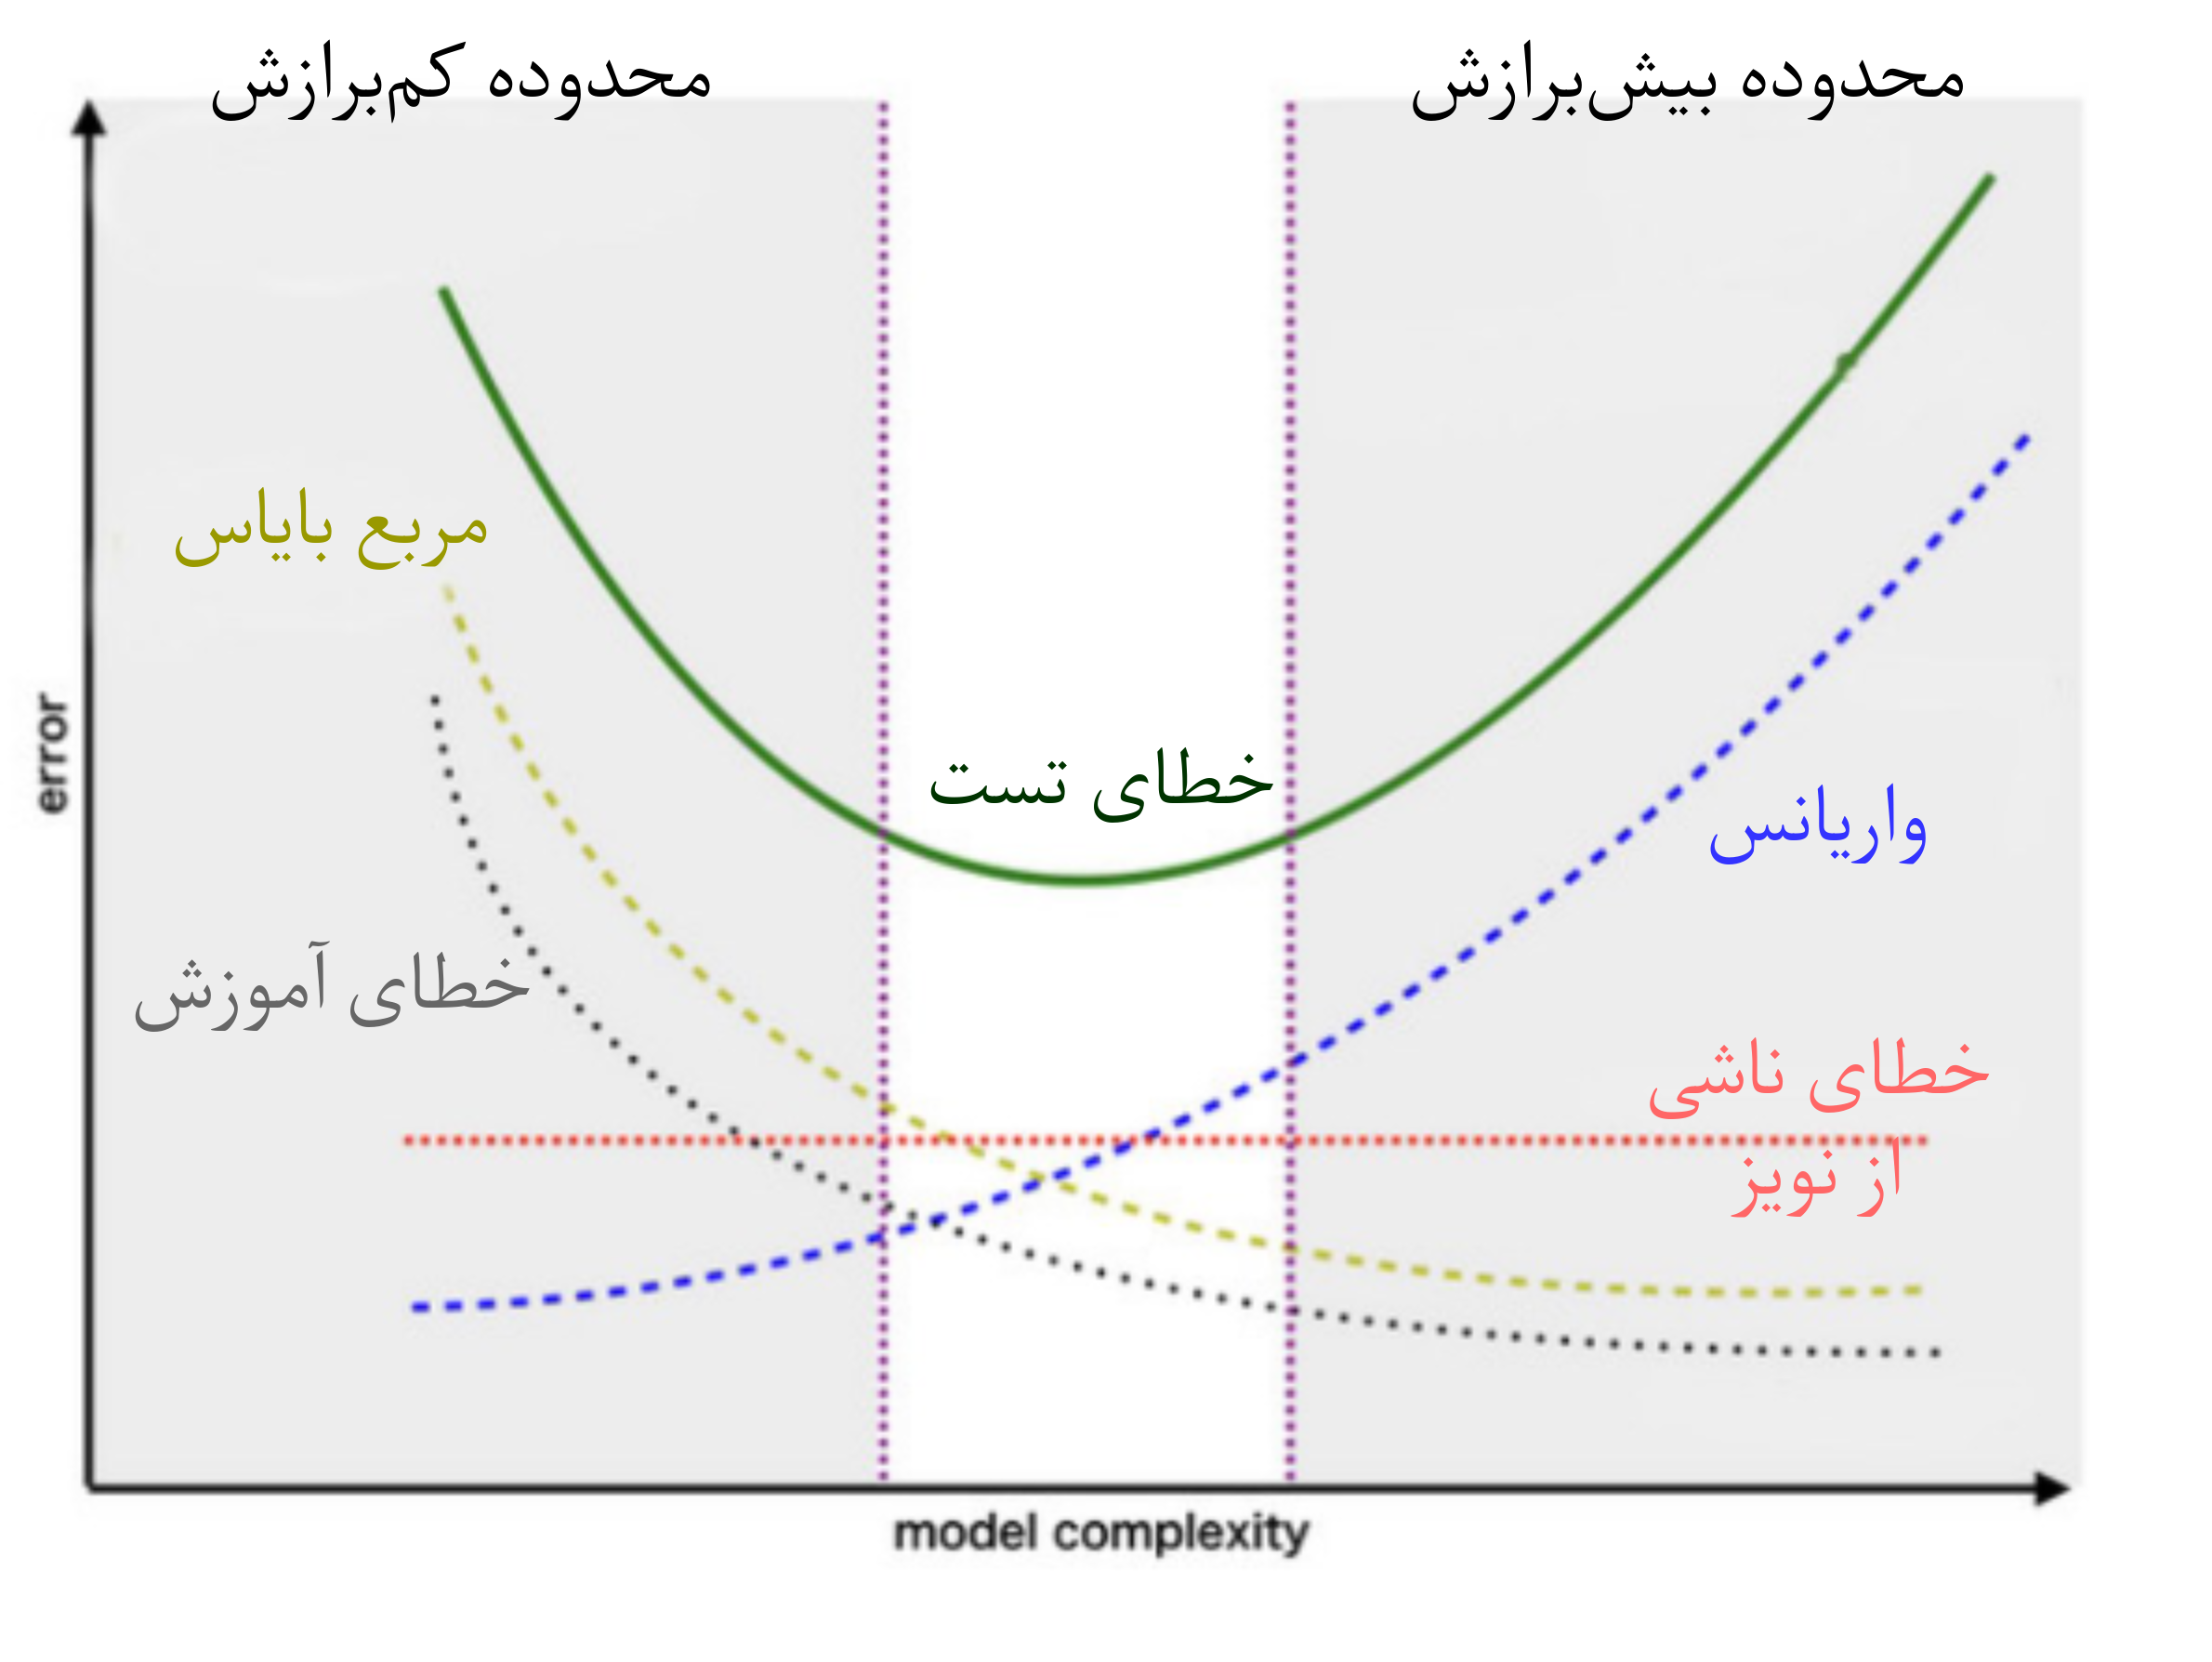
\includegraphics[width=\linewidth]{images/q6.png}
\end{figure}

\newpage

\section*{پیاده‌سازی}

\subsection*{سوال اول}

\subsubsection*{قسمت الف}

در شکل \ref{implementation-q1p1} نمودار داده‌ها مشاهده می‌شود.

\begin{figure}[h]
    \centering
    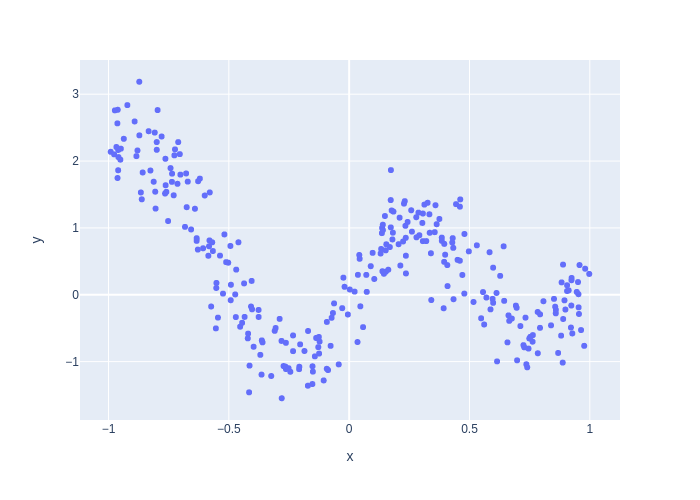
\includegraphics[width=\linewidth]{images/implementation/q1/p1.png}
    \caption{نمودار مربوط به قسمت الف سوال یک قسمت پیاده‌سازی}
    \label{implementation-q1p1}
\end{figure}

\subsubsection*{قسمت ب}

در هنگام تقسیم داده‌ها به دو مجموعه‌ی آموزش و تست، پیش از انجام عمل شافل‌کردن،
ممکن است بخشی از داده‌ها که دارای الگوی واحدی هستند تنها در یکی از مجموعه‌های آموزش و یا تست قرار گیرد.
در نتیجه این اتفاق مدل به دقت خوبی در دادگان آموزشی دست یابد ولی نتواند بر روی داده‌های ارزیابی
به خوبی داده‌های آموزشی عمل کند.

برای بررسی این که آیا داده‌ها به شافل‌کردن نیاز دارند یا خیر، داده‌ها را سطر‌های 1 تا 100 را گروه اول،
سطر‌های 101 تا 200 را گروه دو و سطر‌های 201 تا 300 را گروه سوم در نظر گرفته و هر سه گروه را رسم می‌کنیم.
(شکل \ref{implementation-q1p2}) همان‌طور که مشاهده می‌شود با وجود آن که داده‌ها
به صورت متوالی به سه قسمت تقسیم شده‌اند اما توزیع آن‌ها تقریبا یکسان است و در نتیجه نیازی به شافل‌کردن نیست.

\begin{figure}[h]
    \centering
    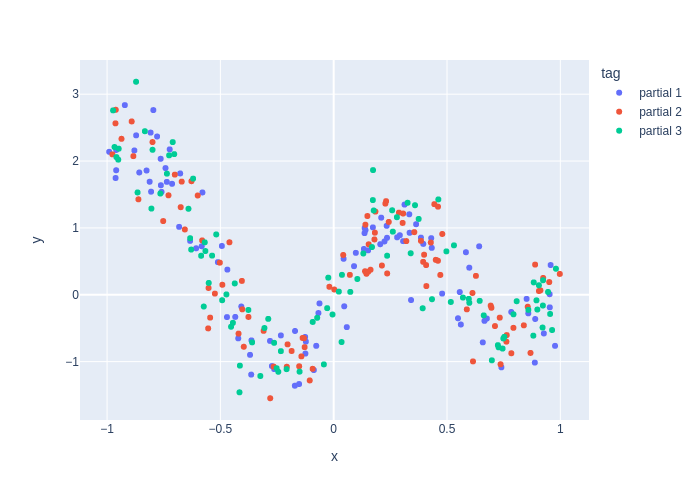
\includegraphics[width=\linewidth]{images/implementation/q1/p2.png}
    \caption{نمودار مربوط به قسمت ب سوال یک قسمت پیاده‌سازی}
    \label{implementation-q1p2}
\end{figure}

\newpage

\subsubsection*{قسمت ج}

در این سوال ۸۰ درصد داده‌ها به عنوان داده آموزشی و ۲۰ درصد داده‌ها به عنوان داده تست استفاده شده است.

در شکل \ref{implementation-q1p3} نمودار‌های حاصل از تغییر تعداد تکرار‌ها، درجه چندجمله‌ای و تابع هزینه
مشاهده می‌شود. در ادامه تاثیر هر یک از پارامتر‌های مسئله را بر روی شکل‌ها بررسی می‌کنیم.

\begin{itemize}
    \item درجه چند جمله‌ای:‌ با افزایش درجه چندجمله‌ای با توجه به اشکال به مدل بهتری دست می‌یابیم.
    با توجه به اشکال نمودار مربوط به چندجمله‌ای درجه پنج تقریبا الگوی کلی داده‌ها را پیدا کرده است اما نسبت به
    نمودار‌های چندجمله‌ای درجه هشت از دقت کم‌تری برخوردار است. البته تفاوت مشهودی بین مدل‌های ارائه شده
    توسط چندجمله‌ای درجه ۸ و ۱۰ مشاهده نمی‌شود. همچنین در هنگام استفاده از چندجمله‌ای درجه ۱۰ بیش‌برازشی مشاهده نمی‌شود.
    البته برای تعیین دقیق این که آیا بیش‌برازش رخ داده است یا خیر باید نمودا‌ر‌های رسم شده در قسمت بعدی را بررسی کرد.
    با توجه به نمودار‌های رسم شده در قسمت بعد با توجه به آن که مقدار خطای داده تست و آموزش  نزولی است،
    بنابراین بیش‌برازش صورت نگرفته است.

    \item تعداد تکرار‌ها. به نظر می‌رسد که تعداد ۵۰۰۰ تکرار برای همگرا شدن مدل کافی است چرا که در هنگامی که
    تعداد تکرار‌ها را به ۱۰۰۰۰تا افزایش می‌دهیم تفاوت ملموسی بین مدل‌های ارائه شده حس نمی‌شود.

    \item تابع هزینه. همان طور که در نمودار‌ها مشاهده می‌شود استفاده از تابع‌های هزینه مختلف تفاوت محسوسی در
    مدل ارائه شده ایجاد نمی‌کند.

\end{itemize}

\begin{figure}[h]
    \centering
    \begin{subfigure}{0.3\linewidth}
        \centering
        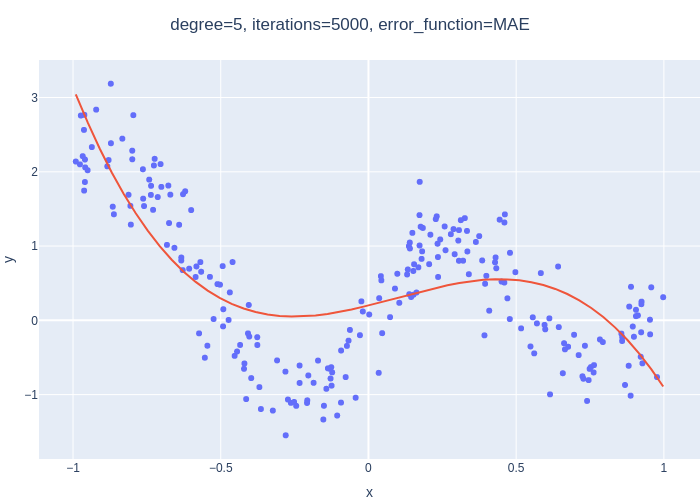
\includegraphics[width=\textwidth]{images/implementation/q1/part_c/5_5000_MAE.png}
    \end{subfigure}
    \hfill
    \begin{subfigure}{0.3\textwidth}
        \centering
        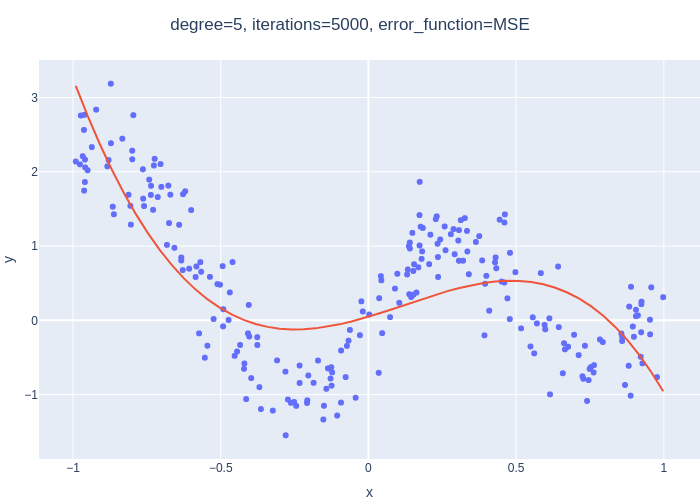
\includegraphics[width=\textwidth]{images/implementation/q1/part_c/5_5000_MSE.png}
    \end{subfigure}
    \hfill
    \begin{subfigure}{0.3\linewidth}
        \centering
        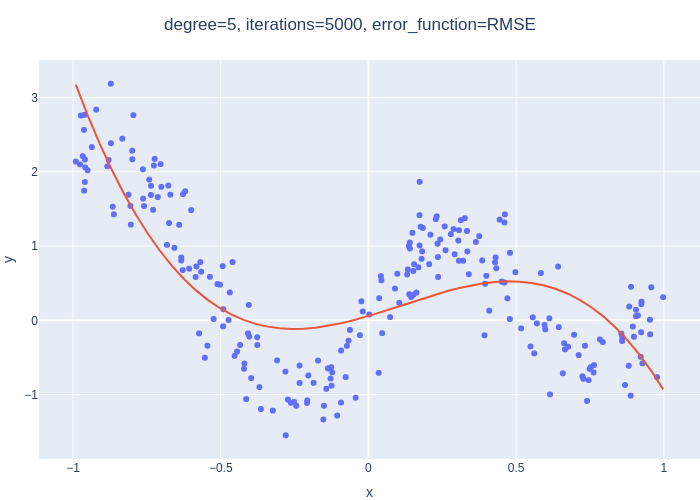
\includegraphics[width=\textwidth]{images/implementation/q1/part_c/5_5000_RMSE.png}
    \end{subfigure}
    \newline
    \begin{subfigure}{0.3\linewidth}
        \centering
        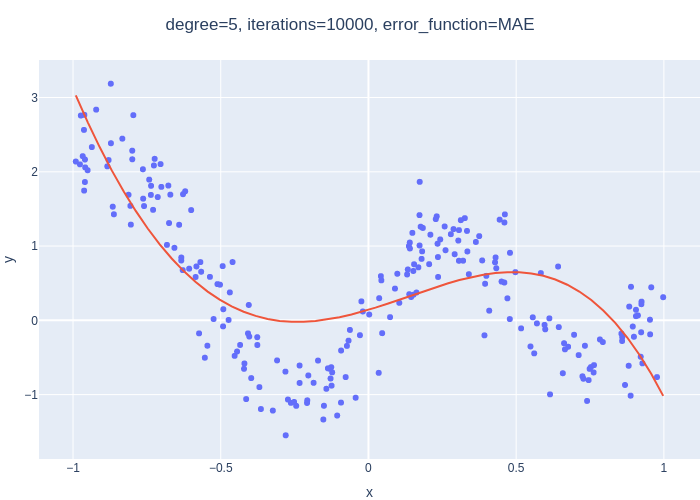
\includegraphics[width=\textwidth]{images/implementation/q1/part_c/5_10000_MAE.png}
    \end{subfigure}
    \hfill
    \begin{subfigure}{0.3\textwidth}
        \centering
        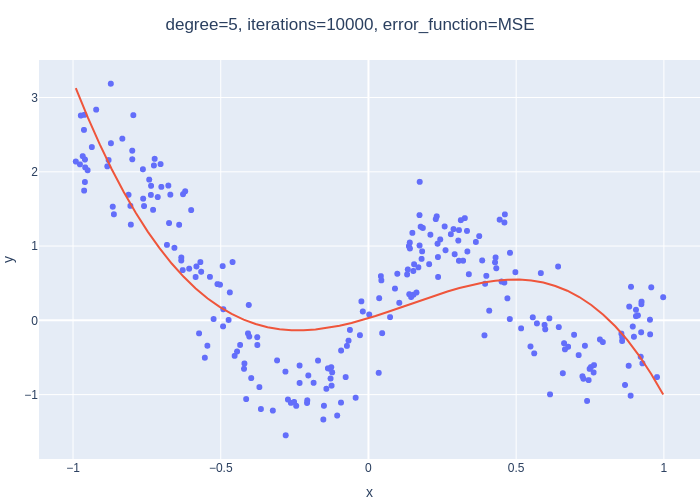
\includegraphics[width=\textwidth]{images/implementation/q1/part_c/5_10000_MSE.png}
    \end{subfigure}
    \hfill
    \begin{subfigure}{0.3\linewidth}
        \centering
        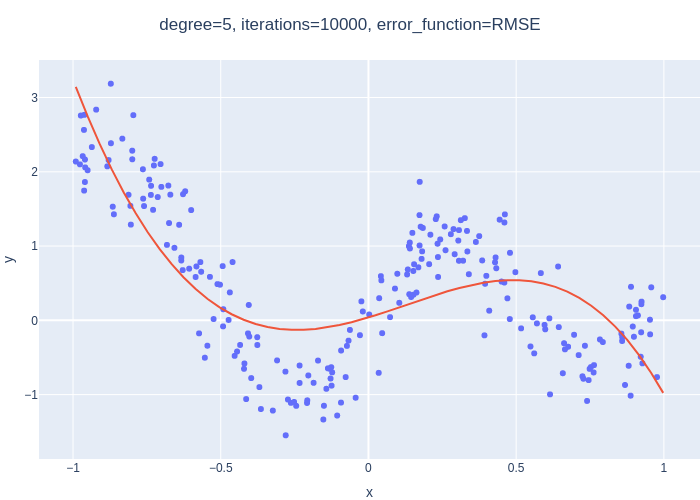
\includegraphics[width=\textwidth]{images/implementation/q1/part_c/5_10000_RMSE.png}
    \end{subfigure}
    \newline
    \begin{subfigure}{0.3\linewidth}
        \centering
        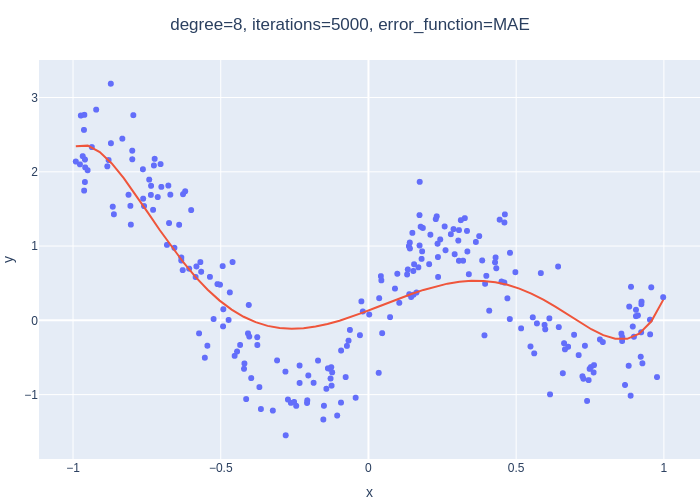
\includegraphics[width=\textwidth]{images/implementation/q1/part_c/8_5000_MAE.png}
    \end{subfigure}
    \hfill
    \begin{subfigure}{0.3\textwidth}
        \centering
        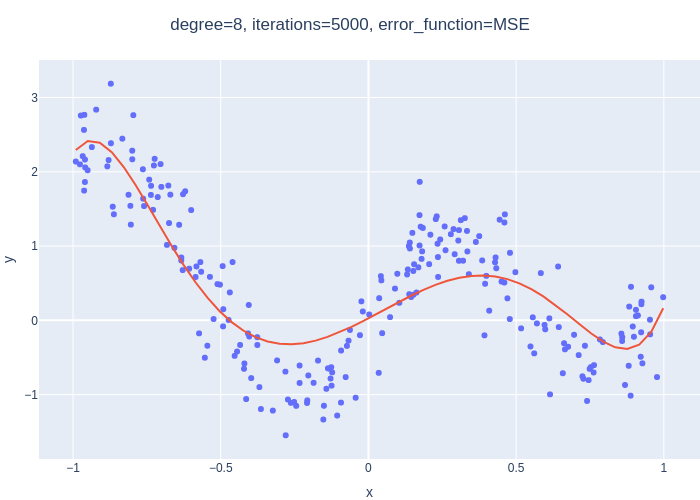
\includegraphics[width=\textwidth]{images/implementation/q1/part_c/8_5000_MSE.png}
    \end{subfigure}
    \hfill
    \begin{subfigure}{0.3\linewidth}
        \centering
        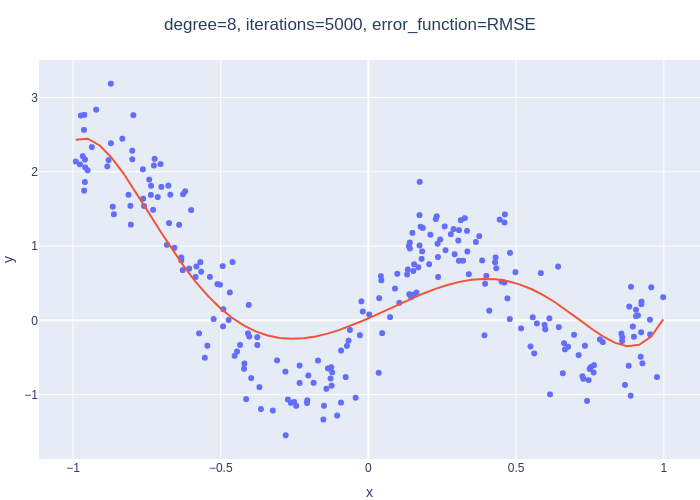
\includegraphics[width=\textwidth]{images/implementation/q1/part_c/8_5000_RMSE.png}
    \end{subfigure}
    \newline
    \begin{subfigure}{0.3\linewidth}
        \centering
        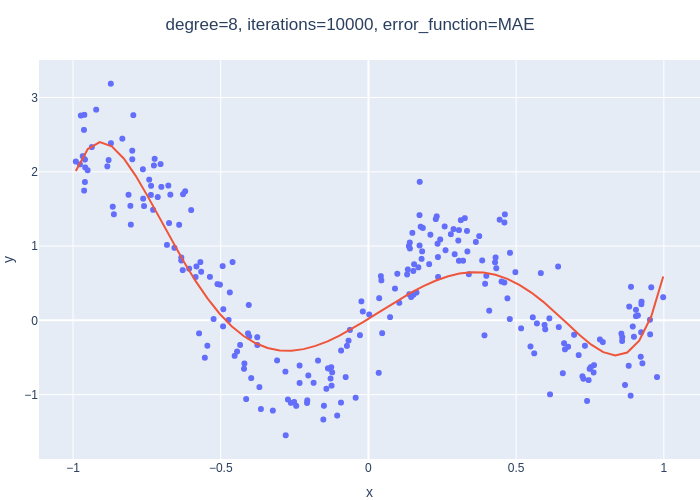
\includegraphics[width=\textwidth]{images/implementation/q1/part_c/8_10000_MAE.png}
    \end{subfigure}
    \hfill
    \begin{subfigure}{0.3\textwidth}
        \centering
        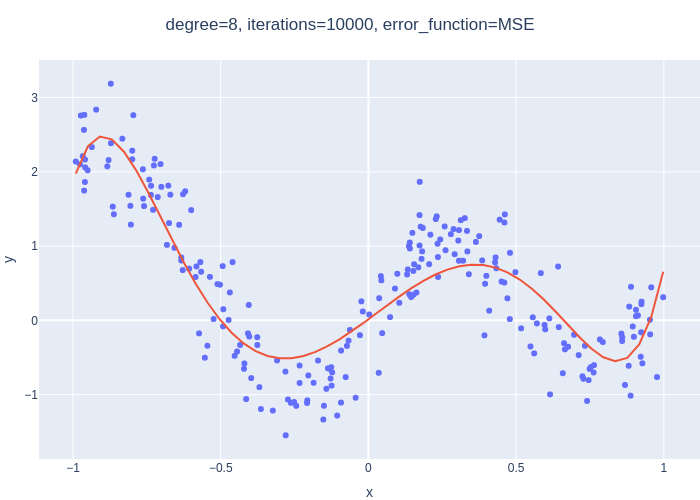
\includegraphics[width=\textwidth]{images/implementation/q1/part_c/8_10000_MSE.png}
    \end{subfigure}
    \hfill
    \begin{subfigure}{0.3\linewidth}
        \centering
        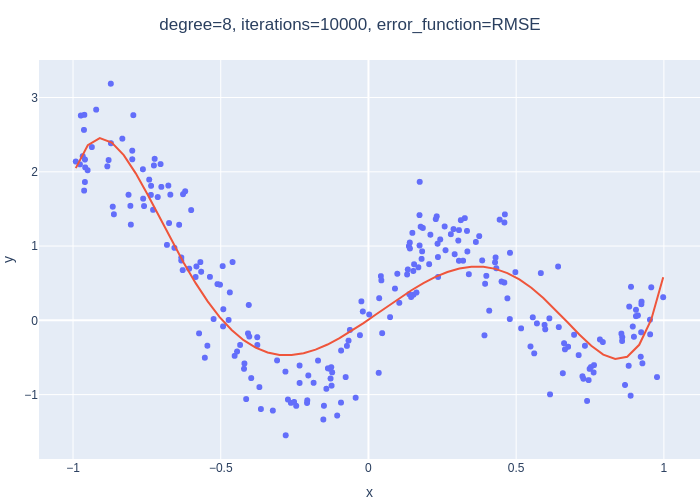
\includegraphics[width=\textwidth]{images/implementation/q1/part_c/8_10000_RMSE.png}
    \end{subfigure}
    \newline
    \begin{subfigure}{0.3\linewidth}
        \centering
        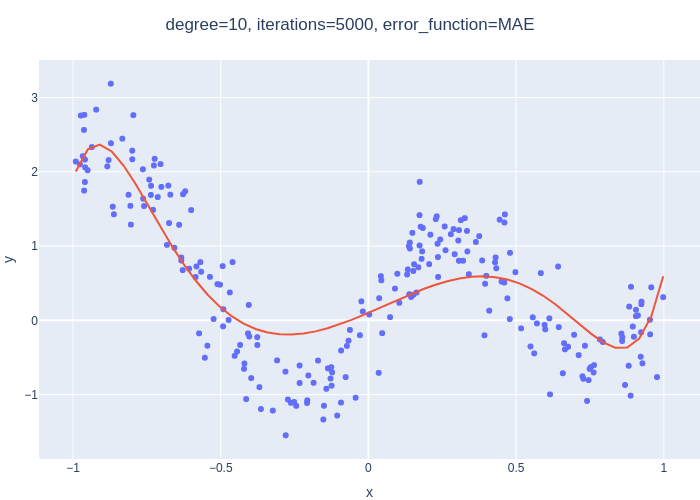
\includegraphics[width=\textwidth]{images/implementation/q1/part_c/10_5000_MAE.png}
    \end{subfigure}
    \hfill
    \begin{subfigure}{0.3\textwidth}
        \centering
        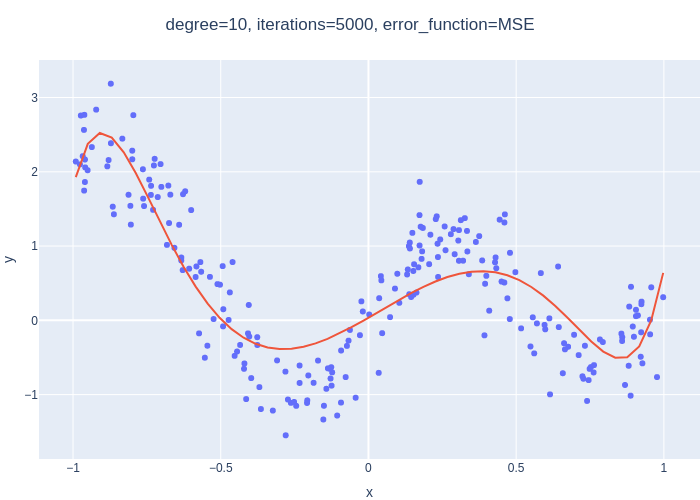
\includegraphics[width=\textwidth]{images/implementation/q1/part_c/10_5000_MSE.png}
    \end{subfigure}
    \hfill
    \begin{subfigure}{0.3\linewidth}
        \centering
        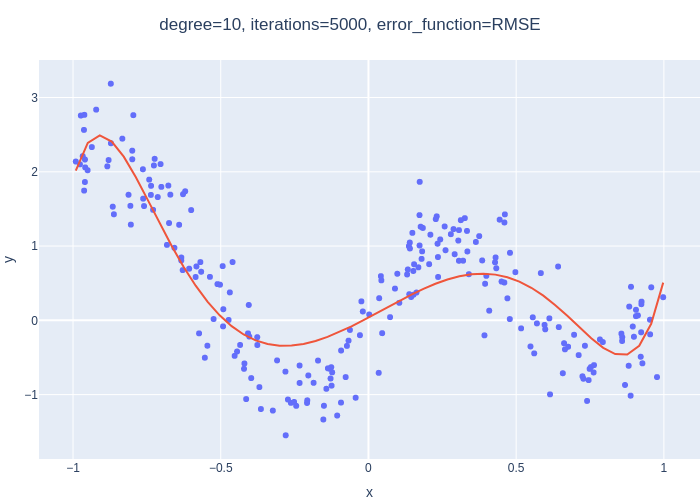
\includegraphics[width=\textwidth]{images/implementation/q1/part_c/10_5000_RMSE.png}
    \end{subfigure}
    \newline
    \begin{subfigure}{0.3\linewidth}
        \centering
        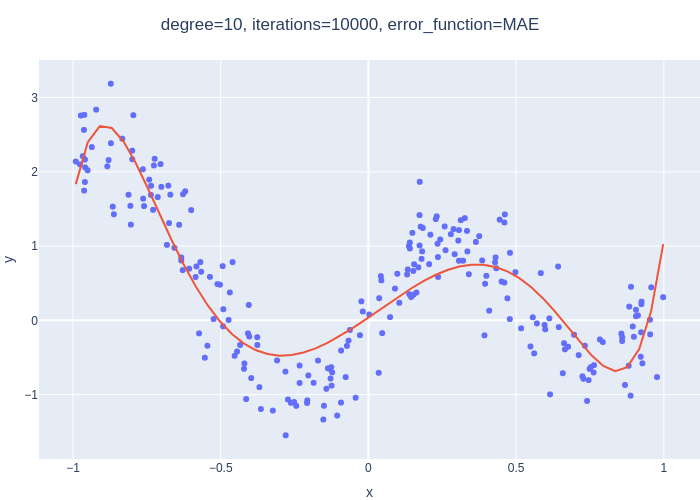
\includegraphics[width=\textwidth]{images/implementation/q1/part_c/10_10000_MAE.png}
    \end{subfigure}
    \hfill
    \begin{subfigure}{0.3\textwidth}
        \centering
        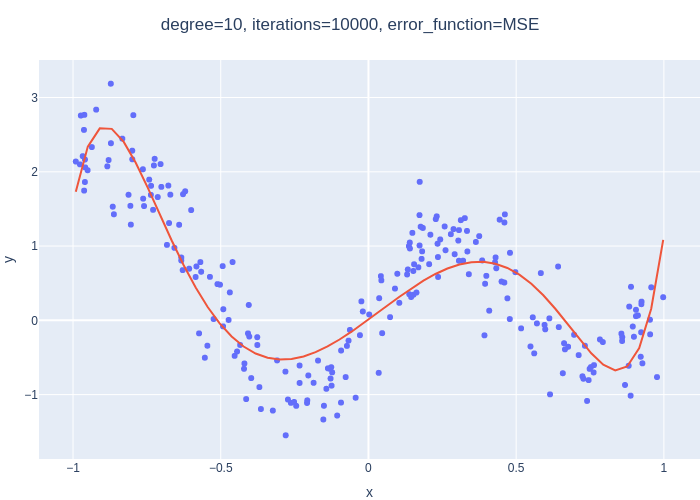
\includegraphics[width=\textwidth]{images/implementation/q1/part_c/10_10000_MSE.png}
    \end{subfigure}
    \hfill
    \begin{subfigure}{0.3\linewidth}
        \centering
        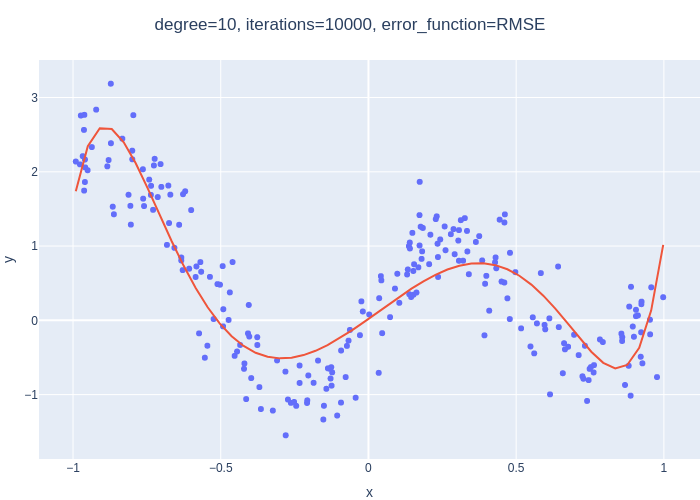
\includegraphics[width=\textwidth]{images/implementation/q1/part_c/10_10000_RMSE.png}
    \end{subfigure}
    \caption{شکل قسمت ج سوال یک پیاده‌سازی}
    \label{implementation-q1p3}
\end{figure}

\newpage

\subsection*{قسمت د}

مجموعه نمودار مربوط به اندازه قدم در شکل \ref{implementation-q1p4-step-size} و مجموعه نمودار
مربوط به خطا در شکل \ref{implementation-q1p4-error} دیده می‌شود.

\begin{figure}[h]
    \centering
    \begin{subfigure}{0.3\linewidth}
        \centering
        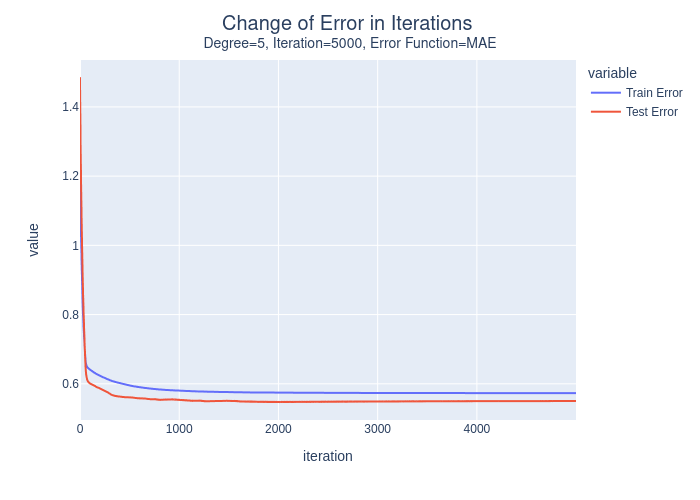
\includegraphics[width=\textwidth]{images/implementation/q1/part_d/error/5_5000_MAE.png}
    \end{subfigure}
    \hfill
    \begin{subfigure}{0.3\textwidth}
        \centering
        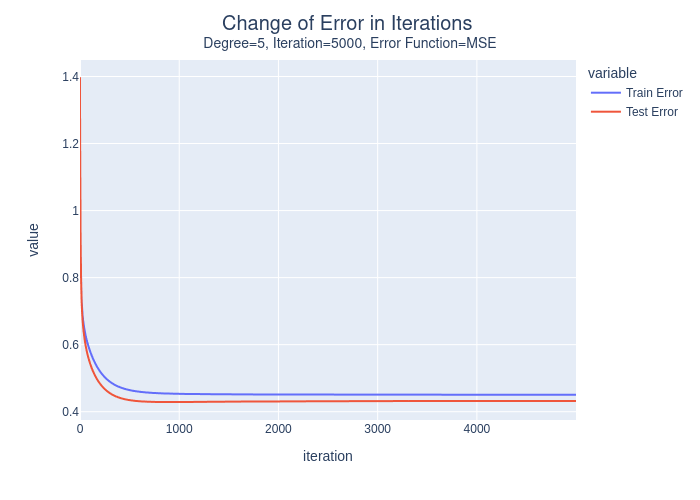
\includegraphics[width=\textwidth]{images/implementation/q1/part_d/error/5_5000_MSE.png}
    \end{subfigure}
    \hfill
    \begin{subfigure}{0.3\linewidth}
        \centering
        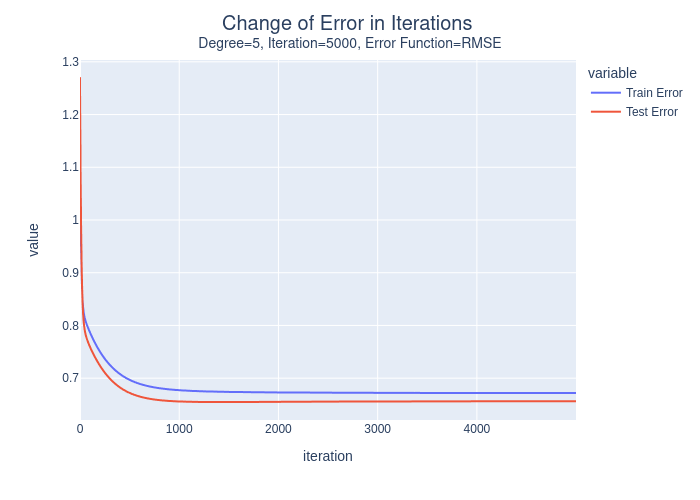
\includegraphics[width=\textwidth]{images/implementation/q1/part_d/error/5_5000_RMSE.png}
    \end{subfigure}
    \newline
    \begin{subfigure}{0.3\linewidth}
        \centering
        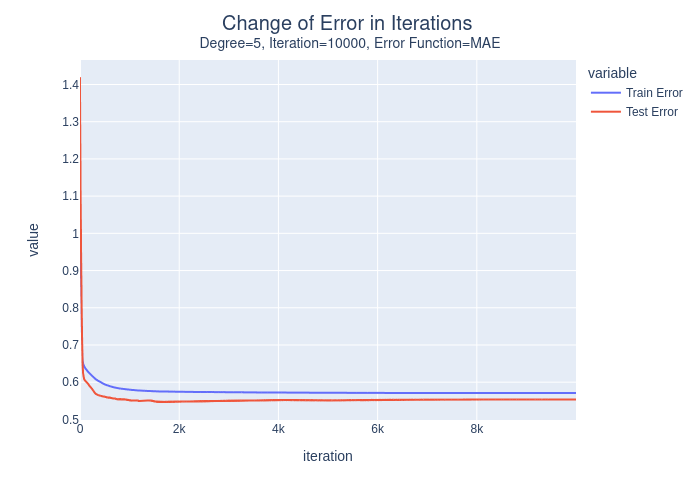
\includegraphics[width=\textwidth]{images/implementation/q1/part_d/error/5_10000_MAE.png}
    \end{subfigure}
    \hfill
    \begin{subfigure}{0.3\textwidth}
        \centering
        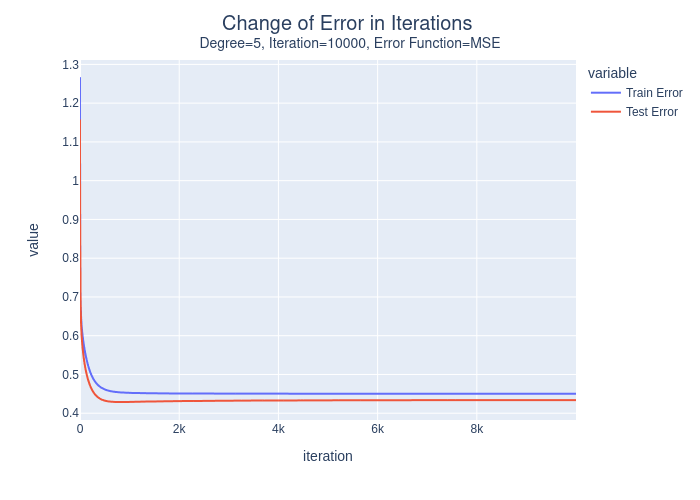
\includegraphics[width=\textwidth]{images/implementation/q1/part_d/error/5_10000_MSE.png}
    \end{subfigure}
    \hfill
    \begin{subfigure}{0.3\linewidth}
        \centering
        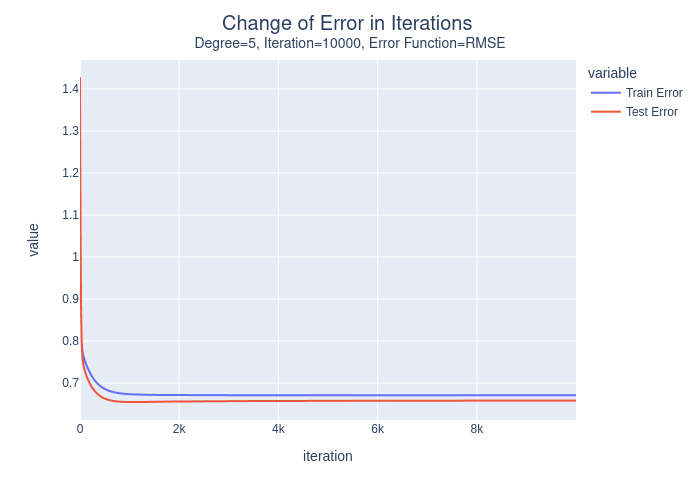
\includegraphics[width=\textwidth]{images/implementation/q1/part_d/error/5_10000_RMSE.png}
    \end{subfigure}
    \newline
    \begin{subfigure}{0.3\linewidth}
        \centering
        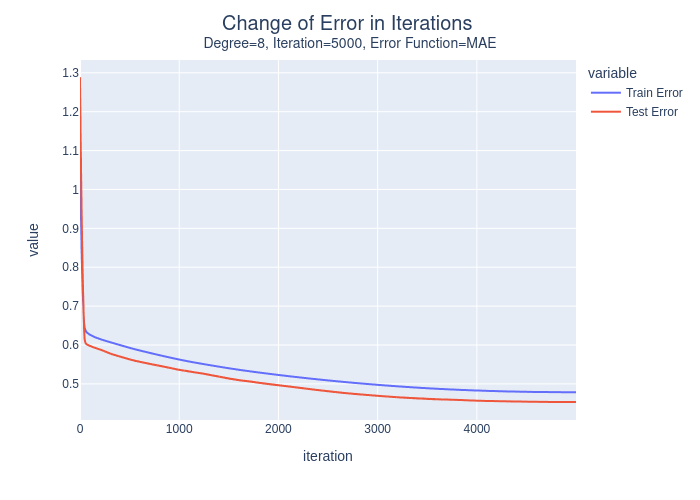
\includegraphics[width=\textwidth]{images/implementation/q1/part_d/error/8_5000_MAE.png}
    \end{subfigure}
    \hfill
    \begin{subfigure}{0.3\textwidth}
        \centering
        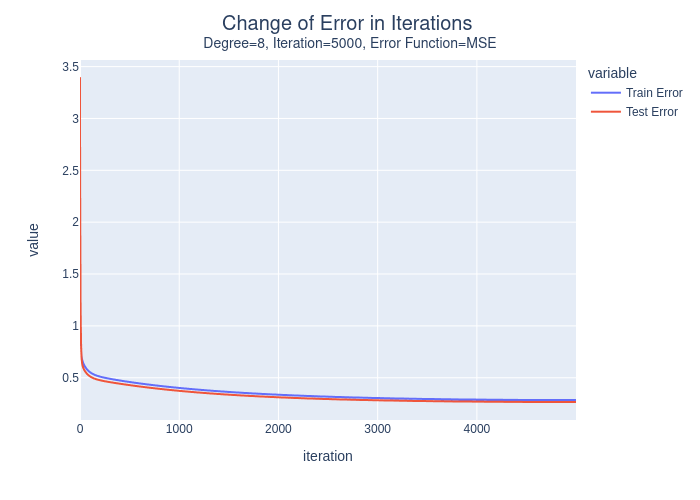
\includegraphics[width=\textwidth]{images/implementation/q1/part_d/error/8_5000_MSE.png}
    \end{subfigure}
    \hfill
    \begin{subfigure}{0.3\linewidth}
        \centering
        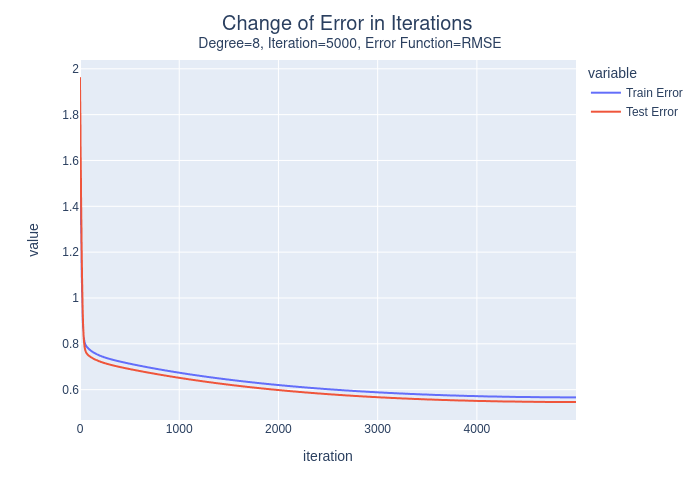
\includegraphics[width=\textwidth]{images/implementation/q1/part_d/error/8_5000_RMSE.png}
    \end{subfigure}
    \newline
    \begin{subfigure}{0.3\linewidth}
        \centering
        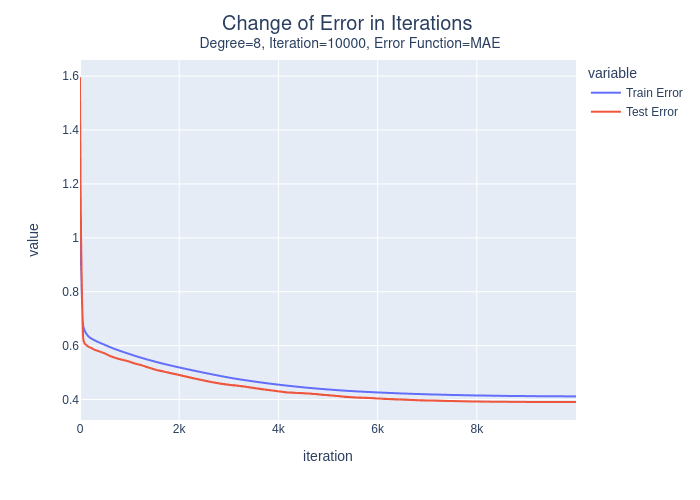
\includegraphics[width=\textwidth]{images/implementation/q1/part_d/error/8_10000_MAE.png}
    \end{subfigure}
    \hfill
    \begin{subfigure}{0.3\textwidth}
        \centering
        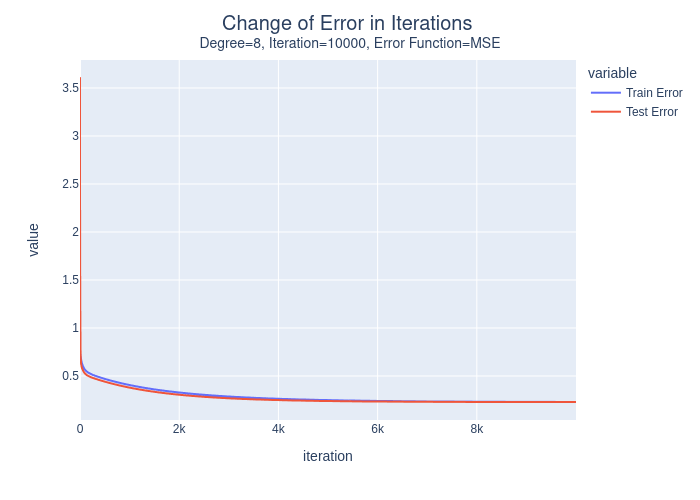
\includegraphics[width=\textwidth]{images/implementation/q1/part_d/error/8_10000_MSE.png}
    \end{subfigure}
    \hfill
    \begin{subfigure}{0.3\linewidth}
        \centering
        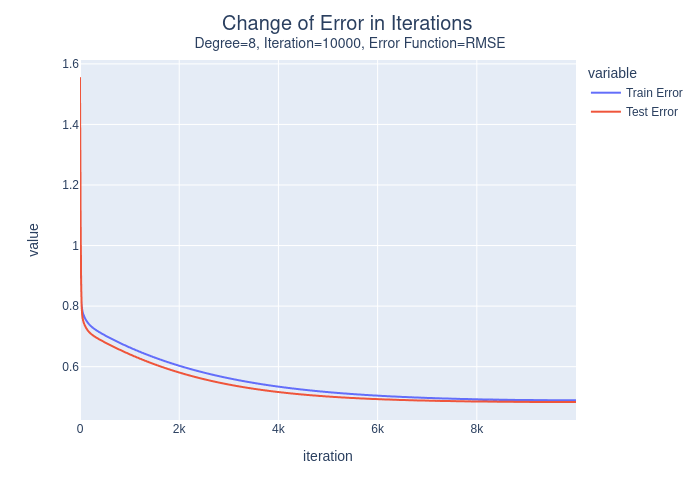
\includegraphics[width=\textwidth]{images/implementation/q1/part_d/error/8_10000_RMSE.png}
    \end{subfigure}
    \newline
    \begin{subfigure}{0.3\linewidth}
        \centering
        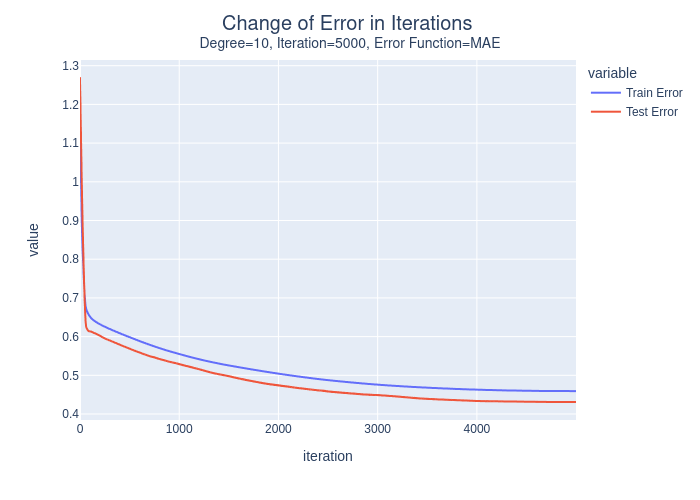
\includegraphics[width=\textwidth]{images/implementation/q1/part_d/error/10_5000_MAE.png}
    \end{subfigure}
    \hfill
    \begin{subfigure}{0.3\textwidth}
        \centering
        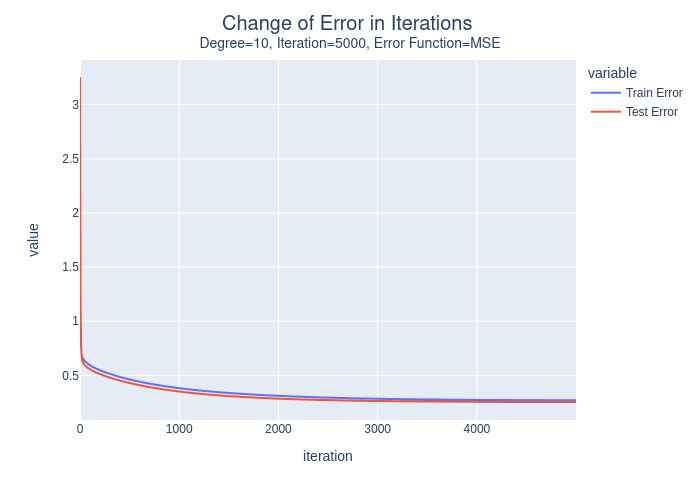
\includegraphics[width=\textwidth]{images/implementation/q1/part_d/error/10_5000_MSE.png}
    \end{subfigure}
    \hfill
    \begin{subfigure}{0.3\linewidth}
        \centering
        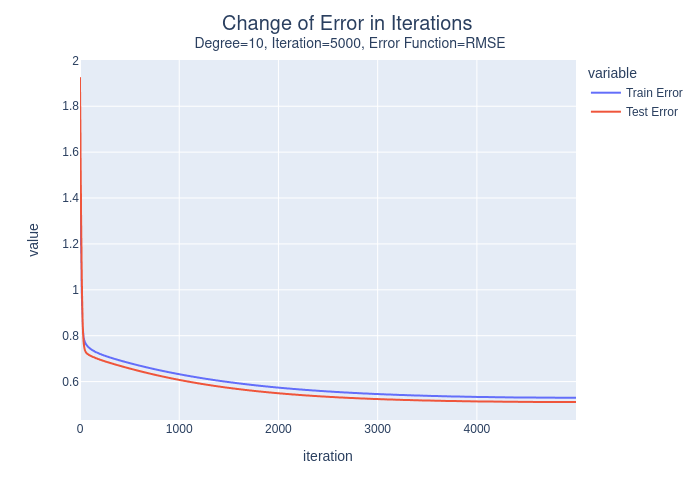
\includegraphics[width=\textwidth]{images/implementation/q1/part_d/error/10_5000_RMSE.png}
    \end{subfigure}
    \newline
    \begin{subfigure}{0.3\linewidth}
        \centering
        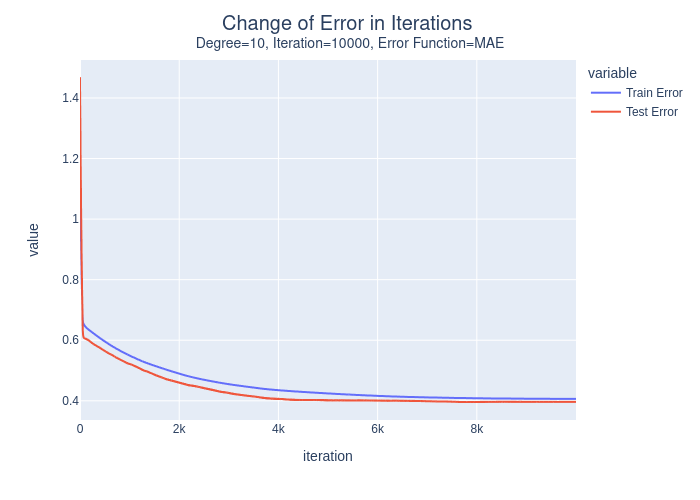
\includegraphics[width=\textwidth]{images/implementation/q1/part_d/error/10_10000_MAE.png}
    \end{subfigure}
    \hfill
    \begin{subfigure}{0.3\textwidth}
        \centering
        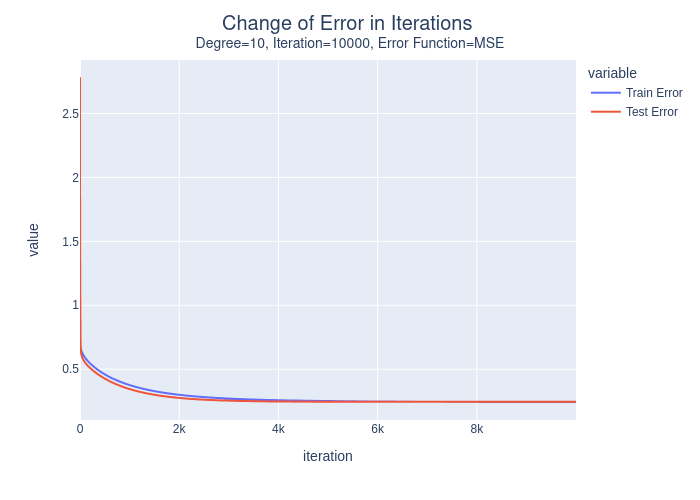
\includegraphics[width=\textwidth]{images/implementation/q1/part_d/error/10_10000_MSE.png}
    \end{subfigure}
    \hfill
    \begin{subfigure}{0.3\linewidth}
        \centering
        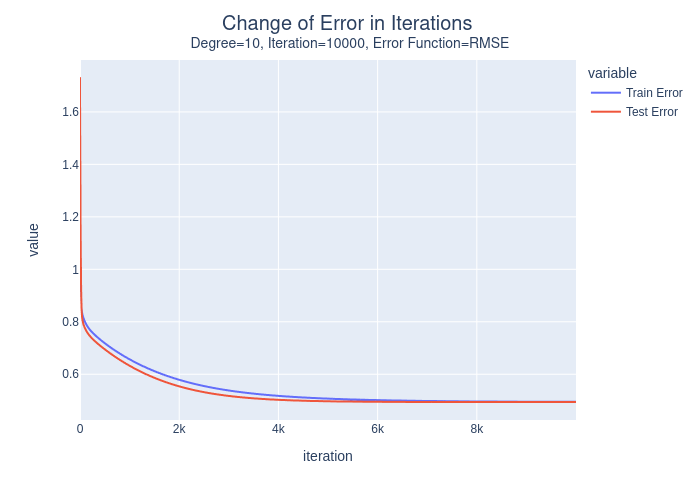
\includegraphics[width=\textwidth]{images/implementation/q1/part_d/error/10_10000_RMSE.png}
    \end{subfigure}
    \caption{شکل قسمت د سوال یک پیاده‌سازی - نمودار خطا در طول آموزش و ارزیابی}
    \label{implementation-q1p4-error}
\end{figure}

\begin{figure}[h]
    \centering
    \begin{subfigure}{0.3\linewidth}
        \centering
        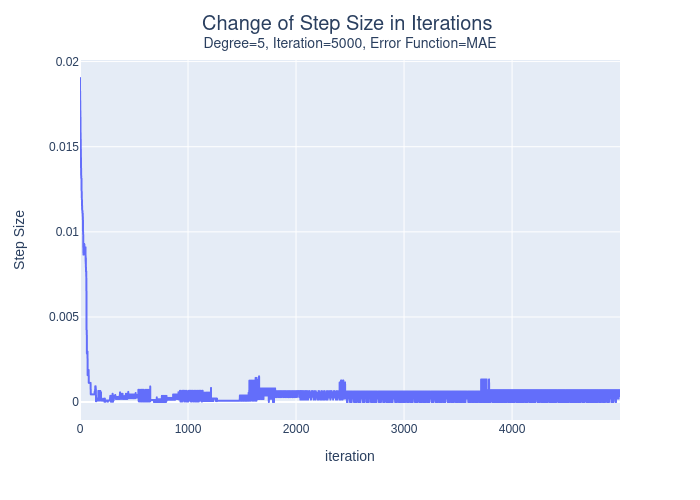
\includegraphics[width=\textwidth]{images/implementation/q1/part_d/step_size/5_5000_MAE.png}
    \end{subfigure}
    \hfill
    \begin{subfigure}{0.3\textwidth}
        \centering
        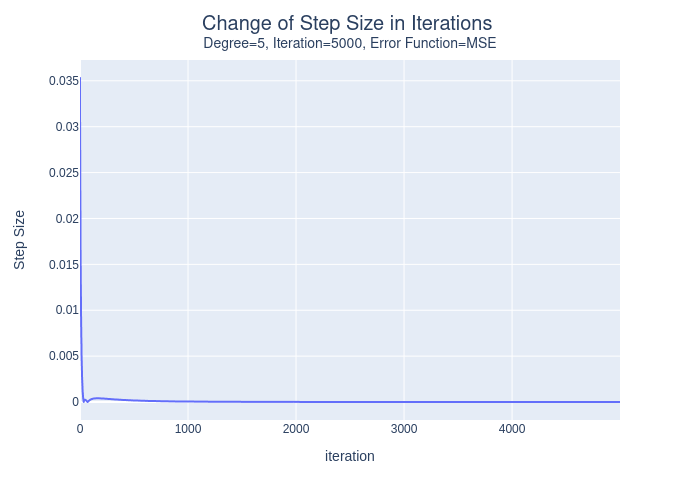
\includegraphics[width=\textwidth]{images/implementation/q1/part_d/step_size/5_5000_MSE.png}
    \end{subfigure}
    \hfill
    \begin{subfigure}{0.3\linewidth}
        \centering
        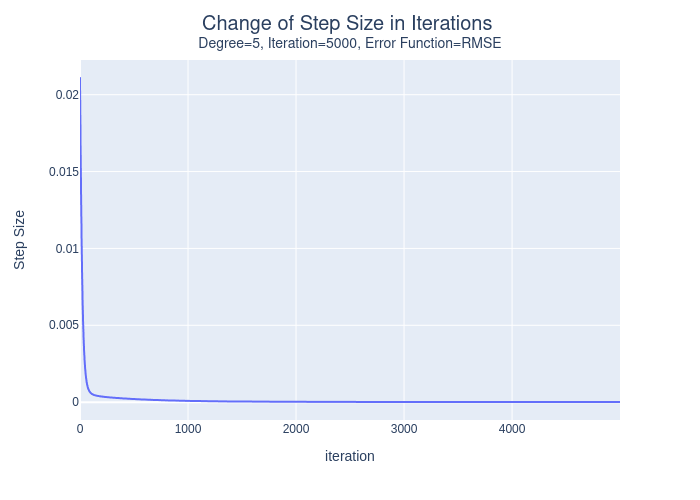
\includegraphics[width=\textwidth]{images/implementation/q1/part_d/step_size/5_5000_RMSE.png}
    \end{subfigure}
    \newline
    \begin{subfigure}{0.3\linewidth}
        \centering
        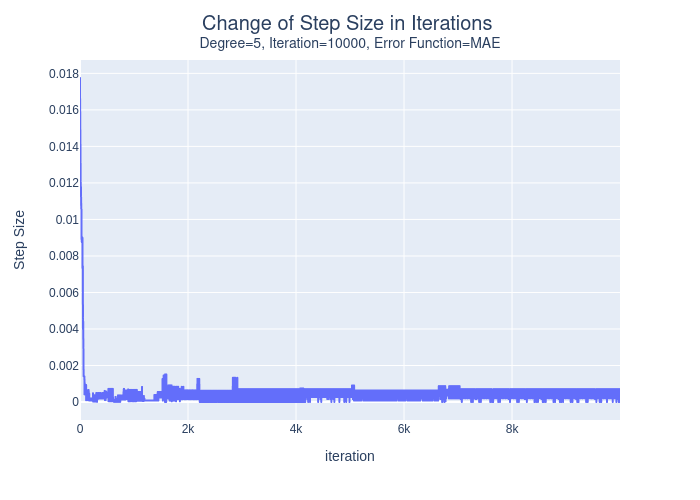
\includegraphics[width=\textwidth]{images/implementation/q1/part_d/step_size/5_10000_MAE.png}
    \end{subfigure}
    \hfill
    \begin{subfigure}{0.3\textwidth}
        \centering
        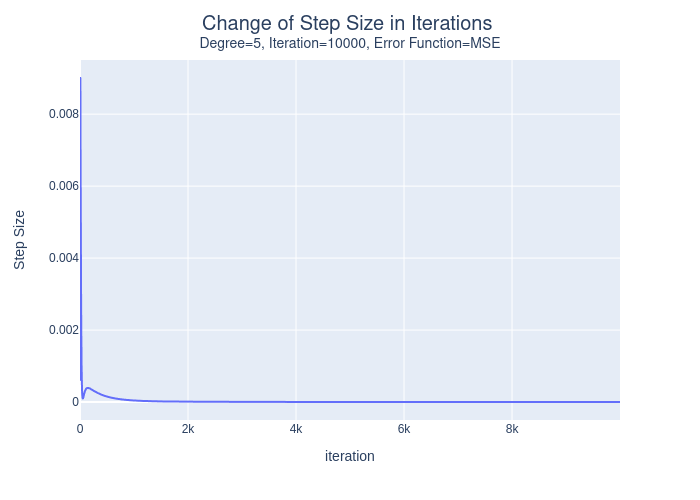
\includegraphics[width=\textwidth]{images/implementation/q1/part_d/step_size/5_10000_MSE.png}
    \end{subfigure}
    \hfill
    \begin{subfigure}{0.3\linewidth}
        \centering
        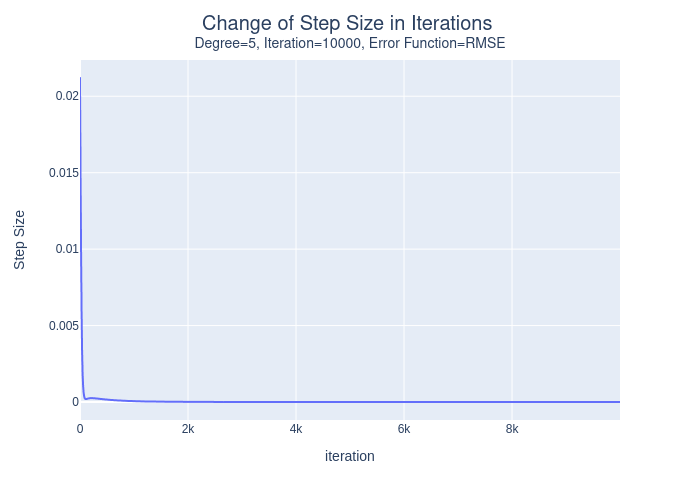
\includegraphics[width=\textwidth]{images/implementation/q1/part_d/step_size/5_10000_RMSE.png}
    \end{subfigure}
    \newline
    \begin{subfigure}{0.3\linewidth}
        \centering
        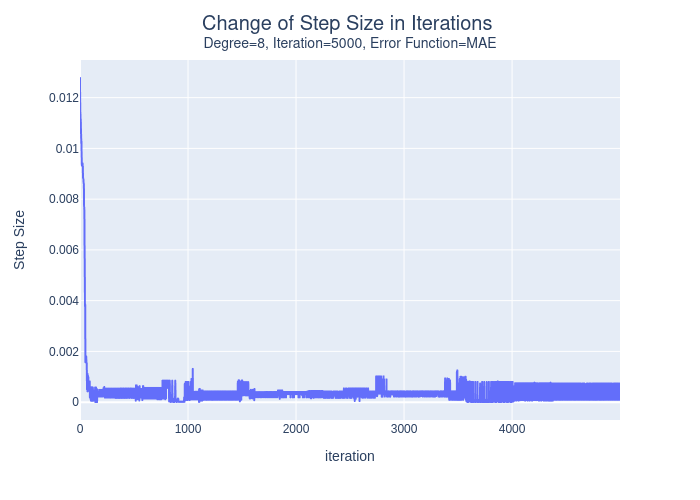
\includegraphics[width=\textwidth]{images/implementation/q1/part_d/step_size/8_5000_MAE.png}
    \end{subfigure}
    \hfill
    \begin{subfigure}{0.3\textwidth}
        \centering
        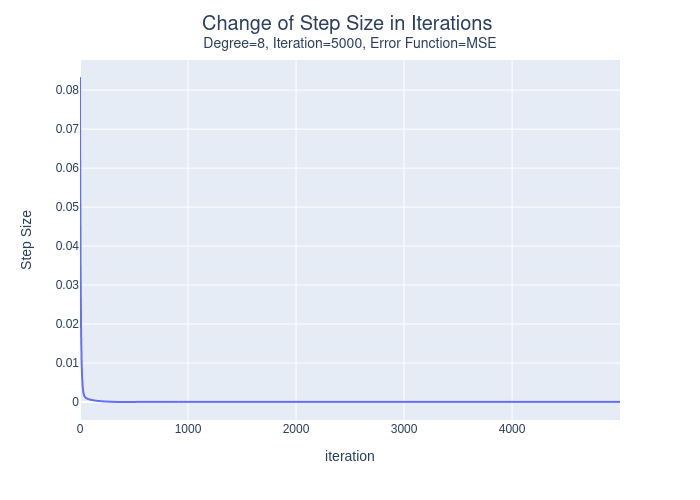
\includegraphics[width=\textwidth]{images/implementation/q1/part_d/step_size/8_5000_MSE.png}
    \end{subfigure}
    \hfill
    \begin{subfigure}{0.3\linewidth}
        \centering
        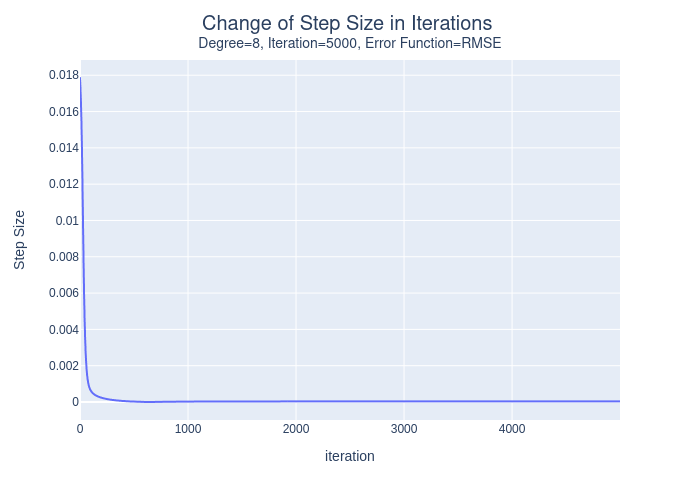
\includegraphics[width=\textwidth]{images/implementation/q1/part_d/step_size/8_5000_RMSE.png}
    \end{subfigure}
    \newline
    \begin{subfigure}{0.3\linewidth}
        \centering
        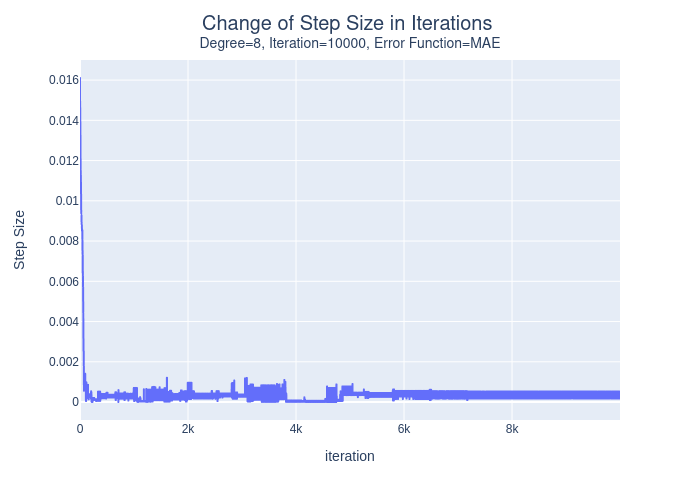
\includegraphics[width=\textwidth]{images/implementation/q1/part_d/step_size/8_10000_MAE.png}
    \end{subfigure}
    \hfill
    \begin{subfigure}{0.3\textwidth}
        \centering
        \includegraphics[width=\textwidth]{images/implementation/q1/part_d/step_size/8_10000_MSE.png}
    \end{subfigure}
    \hfill
    \begin{subfigure}{0.3\linewidth}
        \centering
        \includegraphics[width=\textwidth]{images/implementation/q1/part_d/step_size/8_10000_RMSE.png}
    \end{subfigure}
    \newline
    \begin{subfigure}{0.3\linewidth}
        \centering
        \includegraphics[width=\textwidth]{images/implementation/q1/part_d/step_size/10_5000_MAE.png}
    \end{subfigure}
    \hfill
    \begin{subfigure}{0.3\textwidth}
        \centering
        \includegraphics[width=\textwidth]{images/implementation/q1/part_d/step_size/10_5000_MSE.png}
    \end{subfigure}
    \hfill
    \begin{subfigure}{0.3\linewidth}
        \centering
        \includegraphics[width=\textwidth]{images/implementation/q1/part_d/step_size/10_5000_RMSE.png}
    \end{subfigure}
    \newline
    \begin{subfigure}{0.3\linewidth}
        \centering
        \includegraphics[width=\textwidth]{images/implementation/q1/part_d/step_size/10_10000_MAE.png}
    \end{subfigure}
    \hfill
    \begin{subfigure}{0.3\textwidth}
        \centering
        \includegraphics[width=\textwidth]{images/implementation/q1/part_d/step_size/10_10000_MSE.png}
    \end{subfigure}
    \hfill
    \begin{subfigure}{0.3\linewidth}
        \centering
        \includegraphics[width=\textwidth]{images/implementation/q1/part_d/step_size/10_10000_RMSE.png}
    \end{subfigure}
    \caption{شکل قسمت د سوال یک پیاده‌سازی - نمودار خطا در طول آموزش و ارزیابی}
    \label{implementation-q1p4-step-size}
\end{figure}

\subsection*{قسمت ه}

شکل مربوط به خطای مدل با استفاده از معادله نرمال و روش گرادیان نزولی در شکل \ref{implementation-q1p5} دیده می‌شود.
همان‌طور که انتظار داشتیم، ضرایب به دست آمده با معادله نرمال خطای کمتری نسبت به روش
گرادیان نزولی دارد. دلیل این پدیده روش پیدا کردن کمینه در گرادیان نزولی است. در روش گرادیان نزولی از
یک نقطه تصادفی در فضا شروع کرده و با استفاده از گرادیان به سمت کمینه حرکت می‌کند. از آنجا که
ممکن است کمینه‌ای که گرادیان نزولی به سمت آن حرکت می‌کند، کمینه سراسری نباشد بنابراین خطای به دست آمده
در این روش بیشتر از روش استفاده از معادله نرمال است.

\begin{figure}[h]
    \centering
    \begin{subfigure}{0.45\linewidth}
        \centering
        \includegraphics[width=\textwidth]{images/implementation/q1/part_e/train.png}
    \end{subfigure}
    \hfill
    \begin{subfigure}{0.45\textwidth}
        \centering
        \includegraphics[width=\textwidth]{images/implementation/q1/part_e/test.png}
    \end{subfigure}
    \caption{شکل سوال یک قسمت ه}
    \label{implementation-q1p5}
\end{figure}

\subsection*{قسمت و}

همان‌طور که در مجموعه شکل‌های \ref{implementation-q1p6} دیده می‌شود با اضافه کردن جمله هموار ساز مدل
به دست آمده نرم‌تر می‌شود اما برخلاف انتظار همان‌طور که درشکل \ref{implementation-q1p6-top}
دیده می‌شود، اضافه کردن جمله منظم‌ساز باعث کاهش خطای مدل نشده است.
البته این اتفاق طبیعی است چرا که در  چرا که طبق بررسی‌ها در قسمت‌های قبل، نمودار‌های به دست
آمده بیش برازش نداشته‌اند. بنابراین استفاده از ضریب منظم‌ساز کمکی به کاهش خطای مدل نمی‌کند،
بلکه باعث می‌شود بایاس مدل بیشتر شده و خطا افزایش یابد.

\begin{figure}[h]
    \centering
    \begin{subfigure}{\linewidth}
        \centering
        \includegraphics[width=\textwidth]{images/implementation/q1/part_f.png}
        \caption{تغییرات خطا با تغییر لاندا}
        \label{implementation-q1p6-top}
    \end{subfigure}
    \newline
    \begin{subfigure}{0.3\linewidth}
        \centering
        \includegraphics[width=\textwidth]{images/implementation/q1/part_e/0.01.png}
    \end{subfigure}
    \hfill
    \begin{subfigure}{0.3\textwidth}
        \centering
        \includegraphics[width=\textwidth]{images/implementation/q1/part_e/0.1.png}
    \end{subfigure}
    \hfill
    \begin{subfigure}{0.3\linewidth}
        \centering
        \includegraphics[width=\textwidth]{images/implementation/q1/part_e/0.3.png}
    \end{subfigure}
    \newline
    \begin{subfigure}{0.3\linewidth}
        \centering
        \includegraphics[width=\textwidth]{images/implementation/q1/part_e/0.5.png}
    \end{subfigure}
    \hfill
    \begin{subfigure}{0.3\textwidth}
        \centering
        \includegraphics[width=\textwidth]{images/implementation/q1/part_e/0.7.png}
    \end{subfigure}
    \hfill
    \begin{subfigure}{0.3\linewidth}
        \centering
        \includegraphics[width=\textwidth]{images/implementation/q1/part_e/1.png}
    \end{subfigure}
    \caption{شکل قسمت ه سوال یک پیاده‌سازی }
    \label{implementation-q1p6}
\end{figure}


\newpage

\subsection*{سوال دوم}

\subsubsection*{قسمت الف}

ابتدا ستون‌هایی که مقادیر گمشده وجود دارد را یافته و تعداد آن‌ها را بررسی می‌کنیم.
در جدول زیر تعداد مقادیر گمشده در هر یک از ستون‌ها آورده شده است. برای پر کردن مقادیر گمشده از میانگین
آن‌ ستون استفاده می‌کنیم.

\begin{latin}
    \begin{table}
        \centering
        \begin{tabular}{c|c}
            Column               & \# of missing values \\
            \hline
            Movie                &  0 \\
            Year                 &  0 \\
            Ratings              &  0 \\
            Genre                &  0 \\
            Gross                &  0 \\
            Budget               &  1 \\
            Screens              & 10 \\
            Sequel               &  0 \\
            Sentiment            &  0 \\
            Views                &  0 \\
            Likes                &  0 \\
            Dislikes             &  0 \\
            Comments             &  0 \\
            Aggregate Followers  & 35
        \end{tabular}
    \end{table}
\end{latin}

پیش‌پردازش دیگری که بر روی داده‌ها انجام می‌دهیم، مقیاس داده‌ها به بازه صفر تا یک است. همچنین ستون \lr{Movies}
را نیز با توجه به این که مانند یک شناسه عمل می‌کند و اطلاعاتی را منتقل نمی‌کند حذف می‌کنیم.

\subsubsection*{قسمت ب}

نمودار همبستگی ویژگی‌ها به صورت زیر حاصل می‌شود. (شکل \ref{implementation-q2p2})

\begin{figure}[h]
    \centering
    \includegraphics[width=\linewidth]{images/implementation/q2/part_b.png}
    \caption{شکل سوال ۲ پیاده‌سازی قسمت ب}
    \label{implementation-q2p2}
\end{figure}


\subsubsection*{قسمت ج}

بله، با توجه به نمودار همبستگی می‌توان بعضی از ویژگی‌ها را حذف کرد. ویژگی‌هایی که همبستگی‌ آن‌ها بالای
۷۰ درصد است برای حذف شدن بررسی می‌شوند.

\begin{itemize}
    \item ویژگی‌های \lr{Gross} و \lr{Budget}: از بین این دو ویژگی که ضریب \lr{correlation} بالایی را دارند،
    ویژگی \lr{Budget} را انتخاب می‌کنیم. چرا که این ویژگی \lr{correlation} کم‌تری نسبت ویژگی \lr{Gross} با
    سایر ویژگی‌ها دارد.
    \item ویژگی‌های \lr{Views}، \lr{Likes}، \lr{Dislikes} و \lr{Comments}: از بین این ویژگی‌ها ویژگی \lr{Comments}
    را انتخاب می‌کنیم چرا که نسبت به سایر ویژگی‌ها یعنی \lr{Views}، \lr{Likes}، \lr{Dislikes} ضریب \lr{correlation}
    کم‌تری با تمامی داده‌ها دارد.
\end{itemize}

\subsubsection*{قسمت د}

در این قسمت داده‌های ۸۰ درصد داده‌ها را به عنوان داده آموزشی و ۲۰ درصد داده‌ها را به عنوان داده تست در نظر می‌گیریم.
برای به دست آوردن مدل تعداد \lr{iteration} را برابر ۵۰۰۰ در نظر گرفته‌ایم که با توجه به نمودار‌هایی که در ادامه
رسم می‌شود منطقی به نظر می‌رسد. برای پارامتر $\alpha$ نیز مقدار $0.2$ در نظر گرفته شده است. پارامتر نرخ یادگیری
در طول یادگیری مدل به صورت خطی کاهش داده می‌شود.

\begin{table}
    \centering
    \begin{tabular}{c|c|c}
         & خطای آموزش & خطای ارزیابی  \\
        \hline
        تمامی ویژگی‌ها & $0.026$ & $0.032$ \\
        ویژگی‌های منتخب & $0.029$ & $0.042$
    \end{tabular}
\end{table}


نمودار‌های موجود در شکل \ref{q2-partd-all-features} با استفاده از تمامی داده‌ها رسم شده‌اند.

\begin{figure}[h]
    \centering
     \begin{subfigure}{0.45\linewidth}
         \centering
         \includegraphics[width=\textwidth]{images/implementation/q2/part_d/all_features_error.png}
         \caption{نمودار خطای داده آموزش و ارزیابی}
     \end{subfigure}
     \hfill
     \begin{subfigure}{0.45\textwidth}
         \centering
         \includegraphics[width=\textwidth]{images/implementation/q2/part_d/all_features_step_size.png}
         \caption{نمودار اندازه قدم}
     \end{subfigure}
     \caption{نمودار‌های رسم شده با استفاده از تمامی ویژگی‌ها}
     \label{q2-partd-all-features}
\end{figure}

نمودار‌های موجود در شکل \ref{q2-partd-selected-features} با استفاده از ویژگی‌های منتخب یعنی
\lr{Year}, \lr{Genre}, \lr{Budget}, \lr{Screens}, \lr{Sequel}, \lr{Sentiment}, \lr{Comments}, \lr{Aggregate Followers}
رسم شده‌اند.

\begin{figure}[h]
    \centering
     \begin{subfigure}{0.45\linewidth}
         \centering
         \includegraphics[width=\textwidth]{images/implementation/q2/part_d/selected_feature_error.png}
         \caption{نمودار خطای داده آموزش و ارزیابی}
     \end{subfigure}
     \hfill
     \begin{subfigure}{0.45\textwidth}
         \centering
         \includegraphics[width=\textwidth]{images/implementation/q2/part_d/selected_feature_step_size.png}
         \caption{نمودار اندازه قدم}
     \end{subfigure}
     \caption{نمودار‌های رسم شده با استفاده از ویژگی‌های منتخب}
     \label{q2-partd-selected-features}
\end{figure}


\end{document}